Beim Ausfüllen des UEQ sollten sich die Probanden nur auf den 
Einrichtungsprozess an sich beziehen und auf die Handhabung der 
Blue TOTP App sowie der Blue TOTP Extension. Der Einfluss der 
Website sollte außen vor gelassen werden.
\\\\
Die Verteilung der Antworten zu den Gegensatzpaaren des UEQ sind in Abb. \ref{fig: studie setup ueq dist} zu sehen.
\begin{figure}[h]
    \centering
    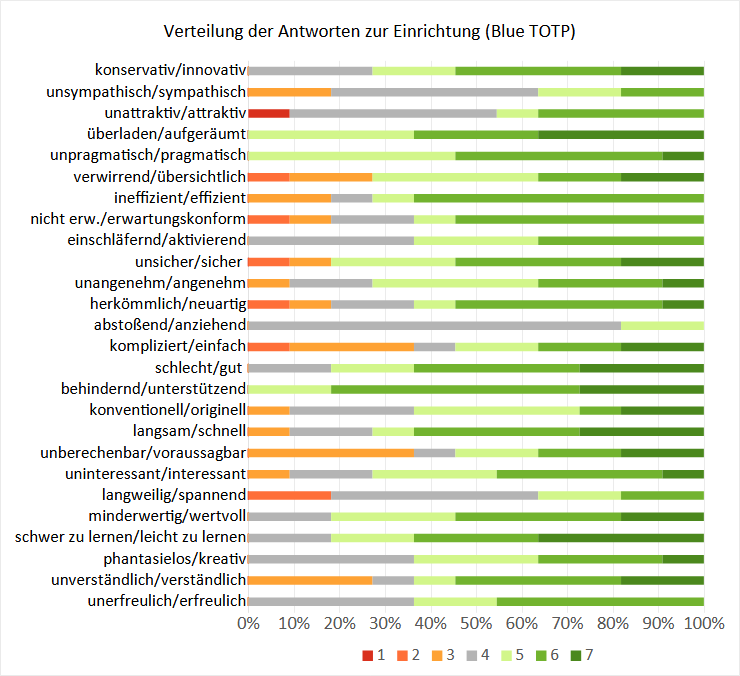
\includegraphics[width=.9\linewidth]{data_processing/questionaires/results/figures_from_excel/setup_ueq_distribution.png}
    \caption[Verteilung der Antworten zum UEQ (Einrichtung Blue TOTP)]{Verteilung der Antworten zum UEQ (Einrichtung Blue TOTP). Die Tendenzen: 1 stärkste Tendenz zum negativen Begriff, 4 neutral, 7 stärkste Tendenz zum positiven Begriff}
    \label{fig: studie setup ueq dist}
\end{figure}
Die Antworten tendieren überwiegend zu den positiven Begriffen 
der Begriffspaare, gefolgt von neutralen Antworten. Die am 
stärksten positiv ausgeprägten Begriffe sind \glqq unterstützend\grqq{} mit 
$\bar{x} = 2{,}1$ und \glqq aufgeräumt\grqq{} mit $\bar{x} = 2{,}0$ (vergl. Anhang 
\ref{anh: studie ergebnisse setup} Tab. \ref{tab: studie setup ueq item 
means}). Interessant  ist die starke Tendenz dahingehend, dass 
das System \glqq leicht zu lernen\grqq{} ($\bar{x} = 1{,}8$) sei, aber es 
dennoch als eher schlecht \glqq voraussagbar\grqq{} ($\bar{x} = 0{,}7$) 
wahrgenommen wird. Zusätzlich dazu überzeugt das System nicht 
sonderlich bzgl. des Paares \glqq einfach/kompliziert\grqq{} mit $\bar{x} = 0.6$.
Das Paar \glqq abstoßend/anziehend\grqq{} wurde beinahe vollständig 
neutral beantwortet, wobei die zwei nicht neutralen Antworten 
direkt an neutral liegen. Das ist ein Indiz dafür, dass die 
Probanden das Begriffspaar nicht mit dem System assoziieren 
können.
\\\\
Durch die Aufteilung der Gegensatzpaare zu ihrer zugehörigen 
Skala (vergl. \autocite[3]{Schrepp}) wurden die in Abb. 
\ref{fig: studie setup ueq overview} dargestellten Mittelwerte 
berechnet. 
\begin{figure}[h!]
    \centering
    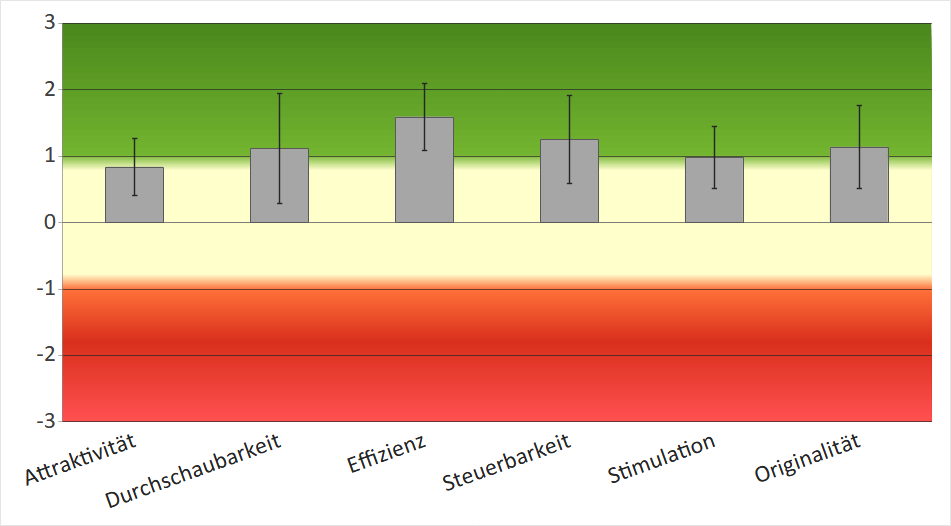
\includegraphics[width=.75\linewidth]{data_processing/questionaires/results/figures_from_excel/setup_ueq_overview.png}
    \caption[Mittelwerte der UEQ-Skalen zur Einrichtung von Blue TOTP]{Mittelwerte der UEQ-Skalen mit 95\%-Konfidenzintervallen zur Einrichtung von Blue TOTP. Farbliche Unterteilung in Bereiche: grün als positiv ($\ge 0.8$), gelb als neutral, rot als negativ ($\le 0.8$)}
    \label{fig: studie setup ueq overview}
\end{figure}
Es ist erkennbar, dass die Einrichtung mit Blue TOTP im Mittel 
bei der Skala Effizienz ($\bar{x} = 1{,}59$) die markanteste Stärke 
besitzt. Auch die Steuerbarkeit ($\bar{x} = 1{,}25$) liegt noch 
deutlich im positiven Bewertungsbereich (größer 0{,}8). Dagegen 
befindet sich die Attraktivität ($\bar{x} = 0{,}83$) auf der Grenze 
zwischen dem neutralen und positiven Bereich. Die verbleibenden 
Skalen Durchschaubarkeit ($\bar{x} = 1{,}11$), Stimulation ($\bar{x} 
= 0{,}98$) und Originalität ($\bar{x} = 1{,}14$) sind nahe über dieser 
Grenze.
\newpage